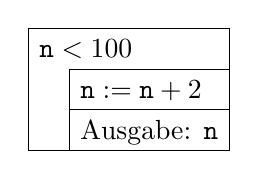
\begin{tikzpicture}
    \draw (0pt,0pt) rectangle (72.58547pt, -44.2243pt);
    \node at (4.0pt, -22.11215pt) {};
    \node at (20.79161pt, -7.4177100000000005pt) {$\texttt{n} < 100$};
    \draw (14.83542pt,-14.83542pt) rectangle (72.58547pt, -29.27986pt);
    \node at (40.751954999999995pt, -22.474304999999998pt) {$\texttt{n} := \texttt{n} + 2$};
    \draw (14.83542pt,-29.27986pt) rectangle (72.58547pt, -44.2243pt);
    \node at (43.710445pt, -37.7243pt) {Ausgabe: $\texttt{n}$};
\end{tikzpicture}
